% Intended LaTeX compiler: pdflatex
\documentclass{article}
\usepackage[utf8]{inputenc}
\usepackage[T1]{fontenc}
\usepackage{graphicx}
\usepackage{longtable}
\usepackage{wrapfig}
\usepackage{rotating}
\usepackage[normalem]{ulem}
\usepackage{amsmath}
\usepackage{amssymb}
\usepackage{capt-of}
\usepackage{hyperref}
\usepackage[spanish]{babel}
\usepackage[usenames,dvipsnames]{color} % Required for custom colors
\renewcommand{\ttdefault}{pcr} % MONOESPACIO CON NEGRIT
\usepackage{lastpage}
\usepackage{listings}
\usepackage{listingsutf8}
\renewcommand{\lstlistingname}{Listado}
\lstset{frame=single,inputencoding=utf8,basicstyle=\scriptsize\ttfamily,showstringspaces=false,numbers=none}
\definecolor{MyDarkGreen}{rgb}{0.0,0.4,0.0} % This is the color used for comments
\lstset{ breaklines=true, postbreak=\mbox{\textcolor{red}{$\hookrightarrow$}\space}, keywordstyle=\bfseries, keywordstyle=[1]\color{Blue}\bfseries,  keywordstyle=[2]\color{Purple}\bfseries,  keywordstyle=[3]\color{Blue}\underbar,   identifierstyle=,   commentstyle=\usefont{T1}{pcr}{m}{sl}\color{MyDarkGreen}\small,   stringstyle=\color{Purple},   showstringspaces=false,   tabsize=2,   morecomment=[l][\color{Blue}]{...} }
\lstset{literate=  {á}{{\'a}}1 {é}{{\'e}}1 {í}{{\'i}}1 {ó}{{\'o}}1 {ú}{{\'u}}1   {Á}{{\'A}}1 {É}{{\'E}}1 {Í}{{\'I}}1 {Ó}{{\'O}}1 {Ú}{{\'U}}1   {à}{{\`a}}1 {è}{{\`e}}1 {ì}{{\`i}}1 {ò}{{\`o}}1 {ù}{{\`u}}1   {À}{{\`A}}1 {È}{{\'E}}1 {Ì}{{\`I}}1 {Ò}{{\`O}}1 {Ù}{{\`U}}1   {ä}{{\"a}}1 {ë}{{\"e}}1 {ï}{{\"i}}1 {ö}{{\"o}}1 {ü}{{\"u}}1   {Ä}{{\"A}}1 {Ë}{{\"E}}1 {Ï}{{\"I}}1 {Ö}{{\"O}}1 {Ü}{{\"U}}1   {â}{{\^a}}1 {ê}{{\^e}}1 {î}{{\^i}}1 {ô}{{\^o}}1 {û}{{\^u}}1   {Â}{{\^A}}1 {Ê}{{\^E}}1 {Î}{{\^I}}1 {Ô}{{\^O}}1 {Û}{{\^U}}1   {œ}{{\oe}}1 {Œ}{{\OE}}1 {æ}{{\ae}}1 {Æ}{{\AE}}1 {ß}{{\ss}}1   {ű}{{\H{u}}}1 {Ű}{{\H{U}}}1 {ő}{{\H{o}}}1 {Ő}{{\H{O}}}1   {ç}{{\c c}}1 {Ç}{{\c C}}1 {ø}{{\o}}1 {å}{{\r a}}1 {Å}{{\r A}}1   {€}{{\euro}}1 {£}{{\pounds}}1 {«}{{\guillemotleft}}1   {»}{{\guillemotright}}1 {ñ}{{\~n}}1 {Ñ}{{\~N}}1 {¿}{{?`}}1 }
\usepackage{caption}
\usepackage{attachfile}
\usepackage[margin=2.5cm,includeheadfoot,includehead,includefoot]{geometry}
\hypersetup{colorlinks,linkcolor=black}
\usepackage{fancyhdr}
\pagestyle{fancyplain}
\chead{}
\lhead{}
\rhead{}
\cfoot{}
\lfoot{\begin{footnotesize}alvaro.gonzalezsotillo@educa.madrid.org\end{footnotesize}}
\rfoot{\begin{footnotesize}\thepage / \pageref{LastPage}\end{footnotesize}}
\usepackage{svg}
\usepackage{letltxmacro}
\LetLtxMacro{\originalincludegraphics}{\includegraphics}
\renewcommand{\includegraphics}[2][]{\IfFileExists{#2.pdf}{\originalincludegraphics[#1]{#2.pdf}}{\originalincludegraphics[#1]{#2}}}
\LetLtxMacro{\originalincludesvg}{\includesvg}
\renewcommand{\includesvg}[2][]{\IfFileExists{#2.pdf}{\originalincludegraphics[#1]{#2.pdf}}{\originalincludegraphics[#1]{#2.svg.pdf}}}
\usepackage{comment}
\excludecomment{NOTES}
\author{Álvaro González Sotillo}
\date{\today}
<<<<<<< Updated upstream
\title{Estudiar informática}
=======
\title{Estudiar FP\\\medskip
\large  (pulsa n para avanzar, o desplaza con el dedo)}
>>>>>>> Stashed changes
\hypersetup{
 pdfauthor={Álvaro González Sotillo},
 pdftitle={Estudiar informática},
 pdfkeywords={},
 pdfsubject={},
 pdfcreator={Emacs 28.0.50 (Org mode 9.4.6)}, 
 pdflang={Spanish}}
\begin{document}

\maketitle
\captionsetup{font=scriptsize}


<<<<<<< Updated upstream
\section{¿Qué es la informática?}
\label{sec:org0000003}
=======
\section*{Cómo moverse por esta presentación}
\label{sec:org0000000}
\begin{center}
\begin{tabular}{ll}
\hline
Tecla & Acción\\
\hline
\texttt{n} & Avanzar ( \textbf{N} ext )\\
\texttt{p} & Retroceder ( \textbf{P} revious )\\
\texttt{CTRL +} & Más grande\\
\texttt{CTRL -} & Más pequeño\\
\texttt{?} & Mostrar resto de acciones\\
\hline
\end{tabular}
\end{center}



\section*{La Formación Profesional}
\label{sec:org0000012}
\begin{itemize}
\item Estudios o aprendizajes que están encaminados a la inserción laboral
\item Vertiente práctica y cercanía a las empresas
\item La duración de los estudios es más breve que los universitarios
\item La incorporación laboral se puede realizar con mayor rapidez
\item Posibilidad de realizar prácticas en el extranjero
\end{itemize}


\subsection*{Acceso}
\label{sec:org0000003}
\begin{center}
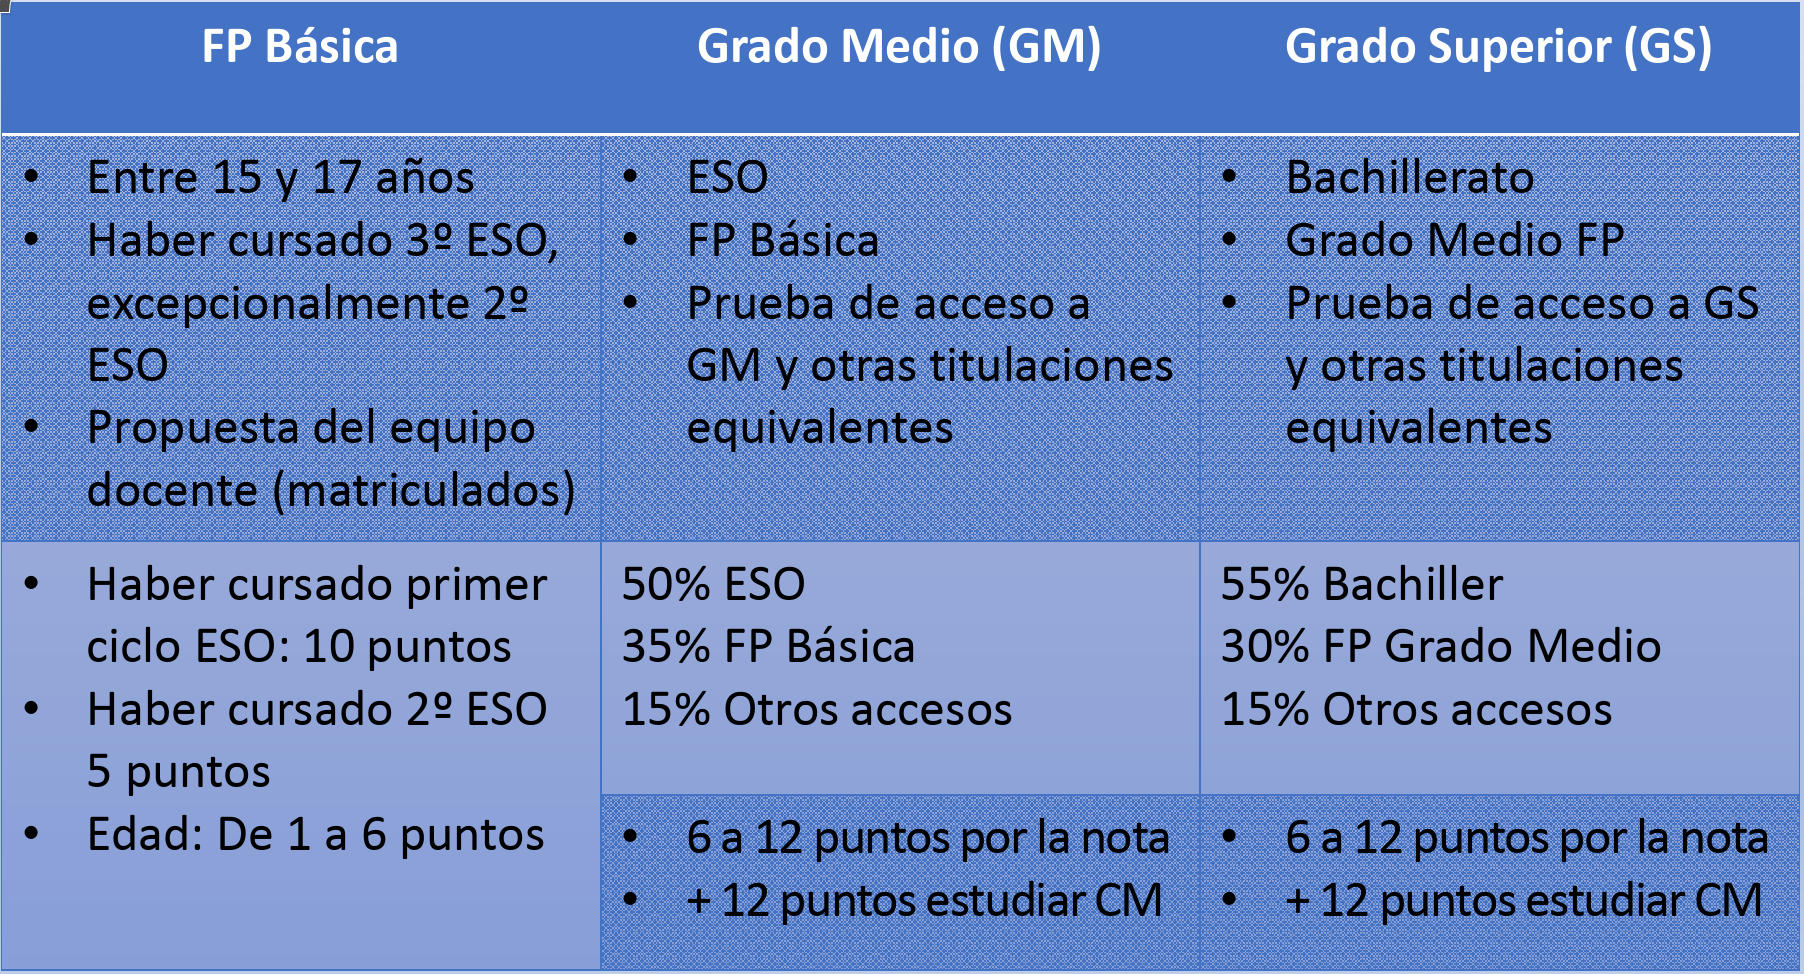
\includegraphics[width=.9\linewidth]{requisitos-y-baremo-acceso.png}
\end{center}

\subsection*{Inserción laboral Grado Medio (2018)}
\label{sec:org0000006}
\begin{center}
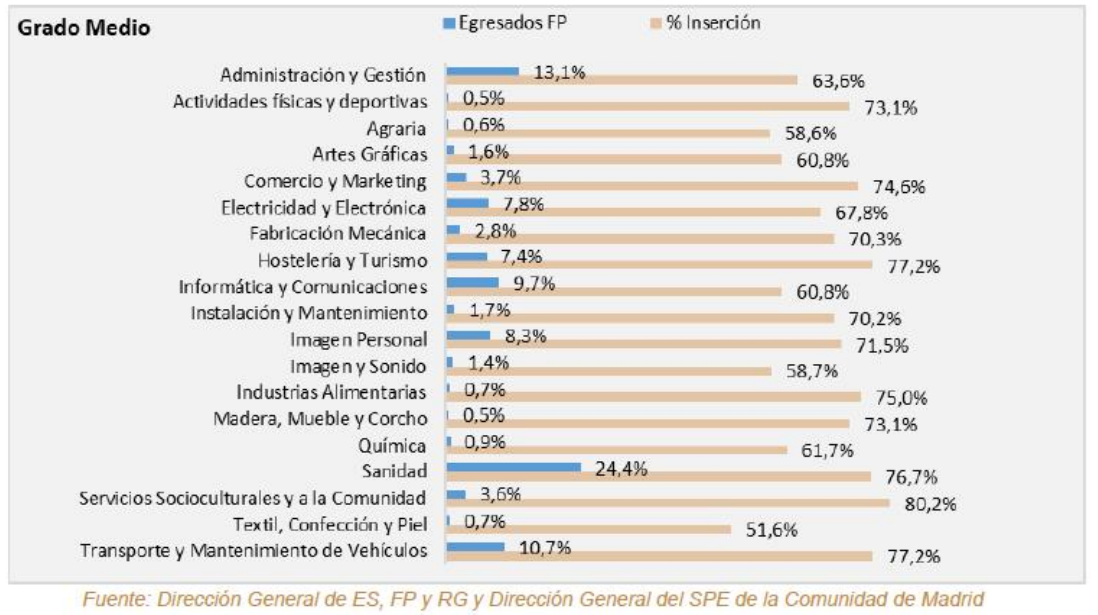
\includegraphics[width=.9\linewidth]{insercion-laboral-2018-grado-medio.png}
\end{center}


\subsection*{Inserción laboral Grado Superior (2018)}
\label{sec:org0000009}
\begin{center}
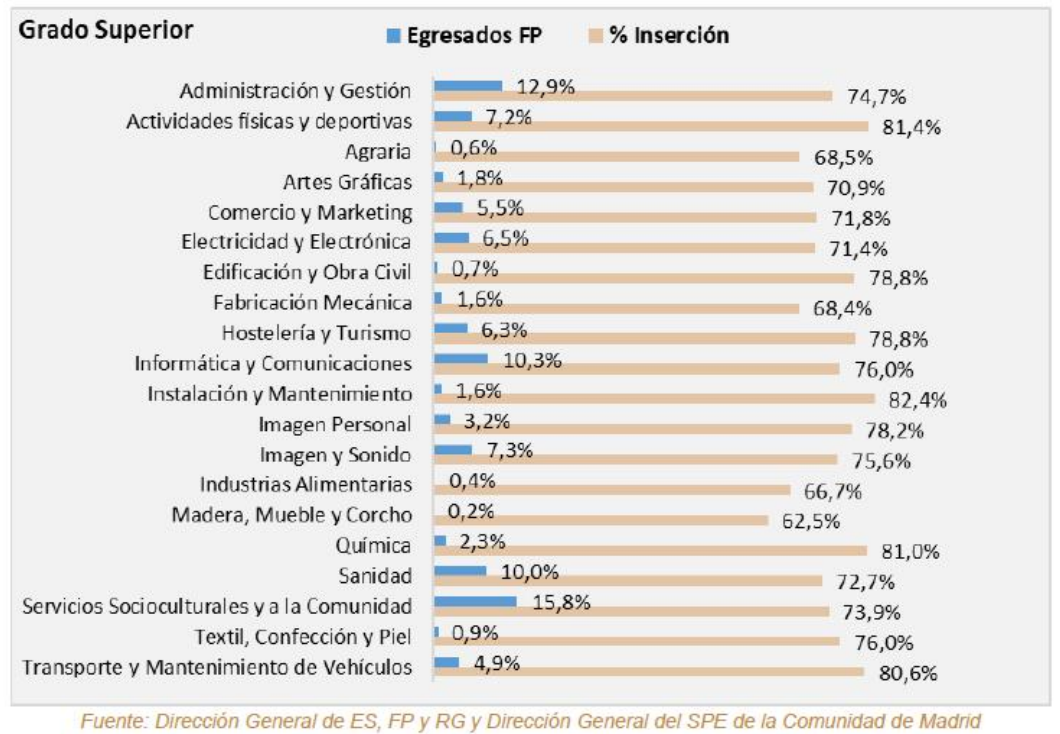
\includegraphics[width=.9\linewidth]{insercion-laboral-2018-grado-superior.png}
\end{center}
\subsection*{Datos actualizados de inserción laboral}
\label{sec:org000000c}
\begin{itemize}
\item Datos generales
\begin{itemize}
\item \url{https://www.educacionyfp.gob.es/servicios-al-ciudadano/estadisticas/laborales/insercion.html}
\end{itemize}
\item Datos de Formación Profesional
\begin{itemize}
\item \url{http://estadisticas.mecd.gob.es/EducaDynPx/educabase/index.htm?type=pcaxis\&path=/laborales/insercion/famprof\&file=pcaxis\&l=s0}
\end{itemize}
\end{itemize}

\subsection*{FP presencial y dual}
\label{sec:org000000f}
\begin{center}
\begin{tabular}{ll}
Presencial & Dual\\
\hline
2 años en el centro & 1 año\\
Prácticas de 1 trimestre & 3 trimestres\\
Prácticas no remuneradas & Prácticas remuneradas\\
Módulos en el centro & Módulos entre centro  y empresa\\
\end{tabular}
\end{center}

\section*{La informática, estereotipada}
\label{sec:org0000018}
>>>>>>> Stashed changes
\begin{itemize}
\item Whatsapp 📞 , Instagram 📷, Meta ♾️
\item Creadores de contenidos
\item Videojuegos
\item Hackers
\end{itemize}
<<<<<<< Updated upstream

\subsection{Pero también es informática}
\label{sec:org0000000}
=======
\subsection*{Pero también es informática}
\label{sec:org0000015}
>>>>>>> Stashed changes
\begin{itemize}
\item Organizar la información de una empresa en una base de datos
\item Preparar las copias de \emph{backup} de los servidores
\item Gestionar las cuentas de usuario de la empresa, y sus permisos
\item Instalar \emph{drivers} de impresoras y otros dispositivos
\item Desarrollar nuevos programas para ordenador, \emph{tablet}, móvil\ldots{}
\item Crear páginas web, tanto estáticas como dinámicas
\item Integrar diferentes servicios (\emph{API}) proporcionados por servidores externos
\end{itemize}

<<<<<<< Updated upstream
\section{Quién hace qué (muy aproximado)}
\label{sec:org000000c}
=======
\section*{Quién hace qué (muy aproximado)}
\label{sec:org0000021}
>>>>>>> Stashed changes
\begin{center}
\includesvg[width=.9\linewidth]{./quien-hace-que}
\end{center}

<<<<<<< Updated upstream
\subsection{Mantenimiento informático}
\label{sec:org0000006}
=======
\subsection*{Mantenimiento informático}
\label{sec:org000001b}
>>>>>>> Stashed changes
\begin{itemize}
\item Montaje de redes y equipos informáticos
\item Configuración de redes y equipos: usuarios, permisos
\item Despliegue de servicios en red: sitios web, almacenamiento de ficheros, mensajería\ldots{}
\item Tratamiento de datos con programas ofimáticos
\item Soporte a usuarios (ayudar a usar las herramientas)
\item Instalación de \emph{software}, local o en la nube
\item Actualización de la web corporativa
\item Seguridad: \emph{firewall} coroporativo, usuarios y permisos, actualizaciones\ldots{}
\end{itemize}

<<<<<<< Updated upstream
\subsection{Desarrollo informático}
\label{sec:org0000009}
=======
\subsection*{Desarrollo informático}
\label{sec:org000001e}
>>>>>>> Stashed changes
\begin{itemize}
\item Creación de nuevas aplicaciones
\begin{itemize}
\item Escritorio
\item Móvil/tableta
\item Web
\end{itemize}
\item Programación de sistemas: \emph{drivers}, microcontroladores\ldots{}
\item Integración de aplicaciones ya existentes
\item Certificación y pruebas de aplicaciones
\item Mejoras y arreglos de aplicaciones antiguas
\item Dirección de proyectos
\end{itemize}

<<<<<<< Updated upstream
\section{¿Me dedico a la informática?}
\label{sec:org0000018}
=======

\section*{¿Me dedico a la informática?}
\label{sec:org000002d}
>>>>>>> Stashed changes

\begin{center}
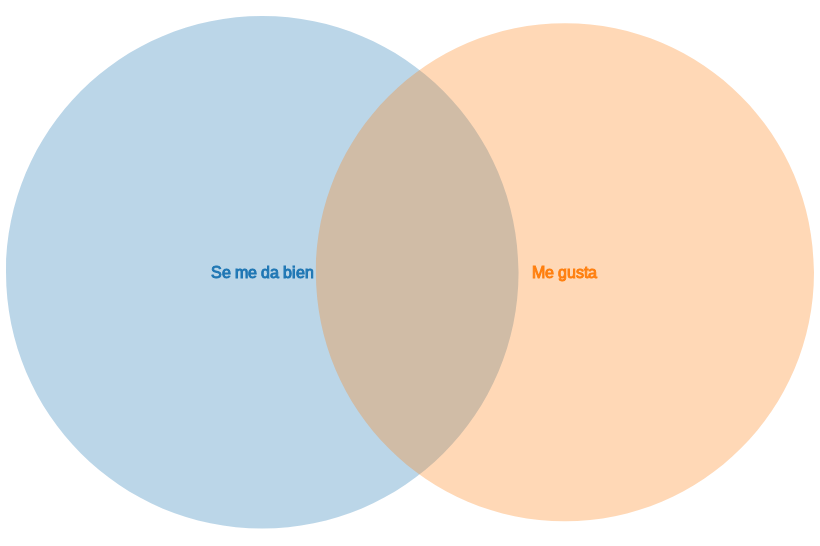
\includegraphics[width=.9\linewidth]{venn-diagram.png}
\end{center}

<<<<<<< Updated upstream
\subsection{Características personales deseables}
\label{sec:org000000f}
=======
\subsection*{Características personales deseables}
\label{sec:org0000024}
>>>>>>> Stashed changes
\begin{itemize}
\item Disposición al autoaprendizaje
\item Organización del trabajo
\item Habilidades interpersonales
\item Habilidades comunicativas
\item Matemáticas, especialmente en el desarrollo de aplicaciones
\item Inglés
\end{itemize}

<<<<<<< Updated upstream

\subsection{Esto no es informática}
\label{sec:org0000012}


\subsection{Cómo saber si me gusta}
\label{sec:org0000015}
=======
\begin{NOTES}
\begin{center}
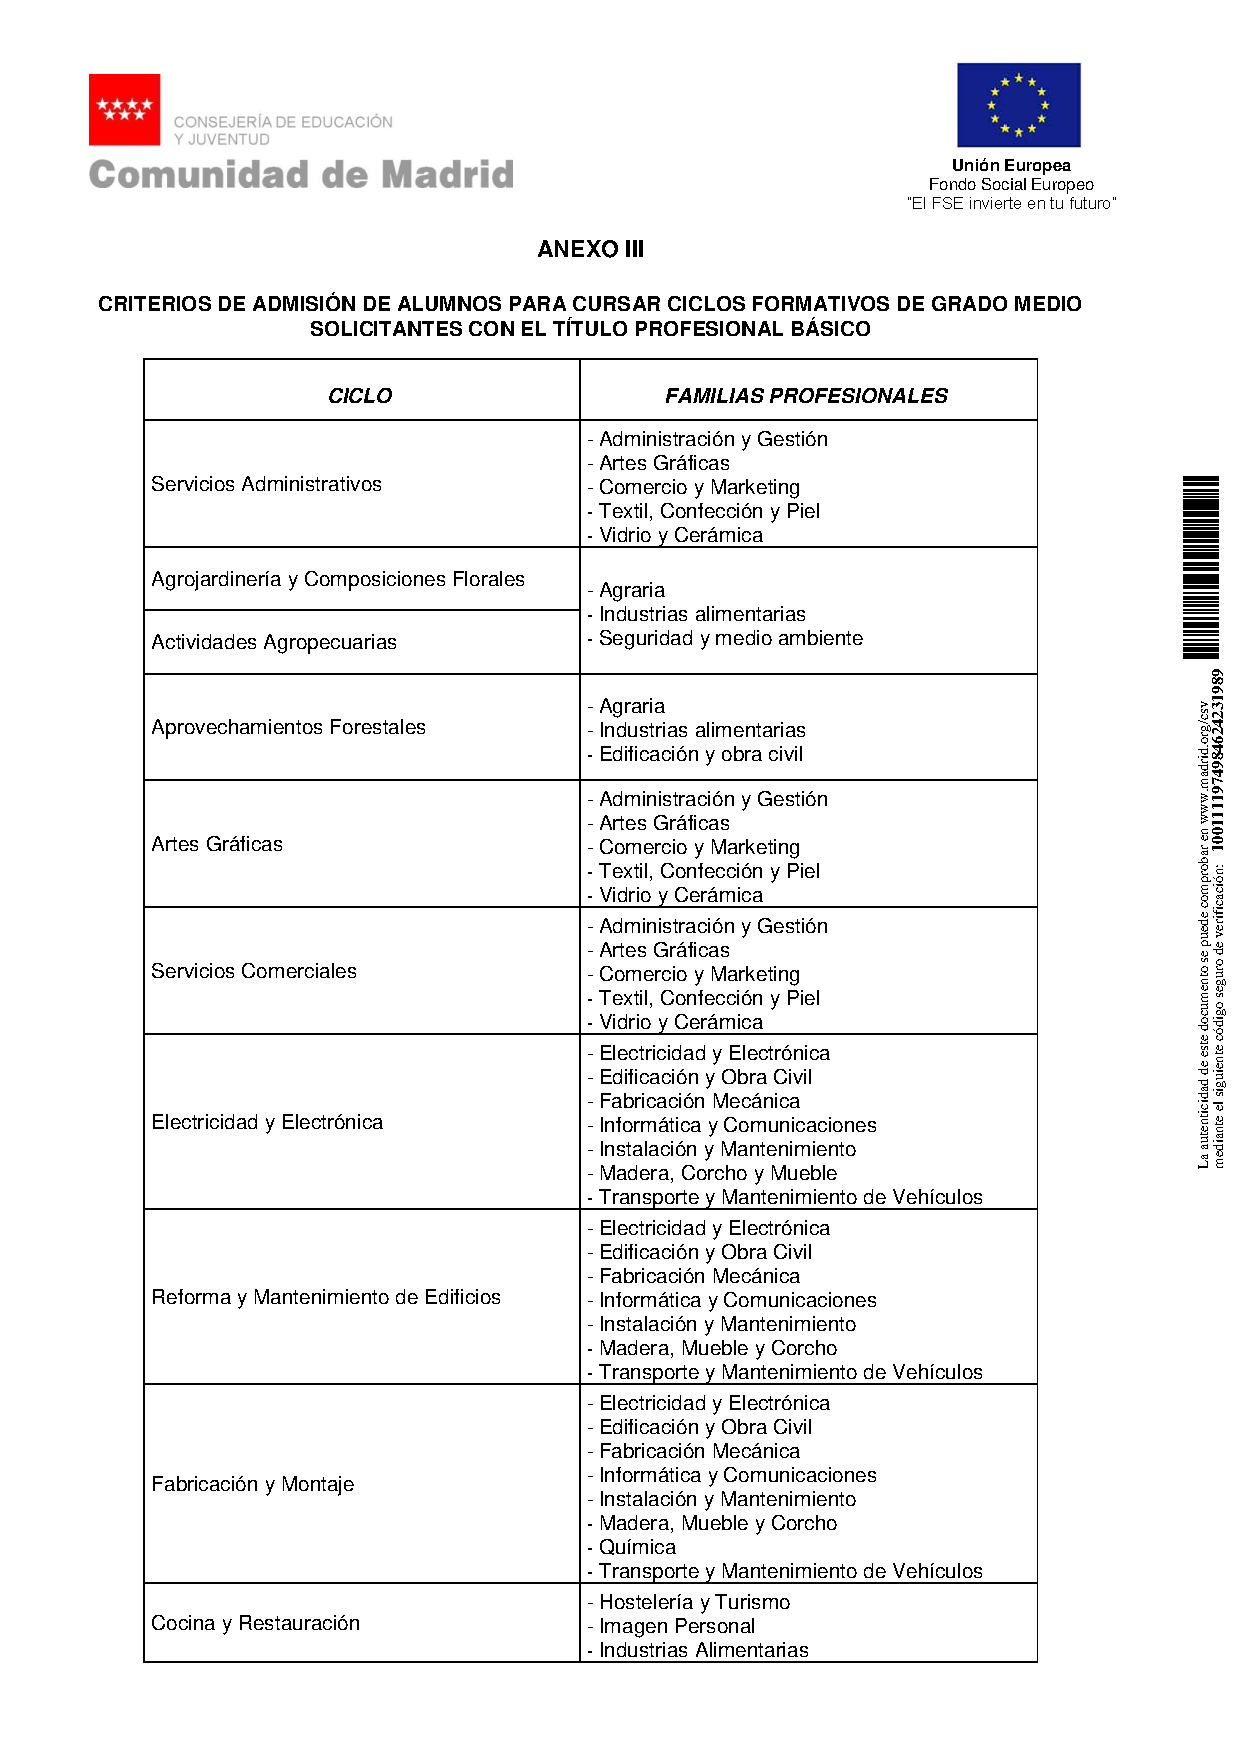
\includegraphics[width=.9\linewidth]{respuestas-posibles-preguntas/preferencias-anexo_iii_gm.pdf}
\end{center}
\begin{center}
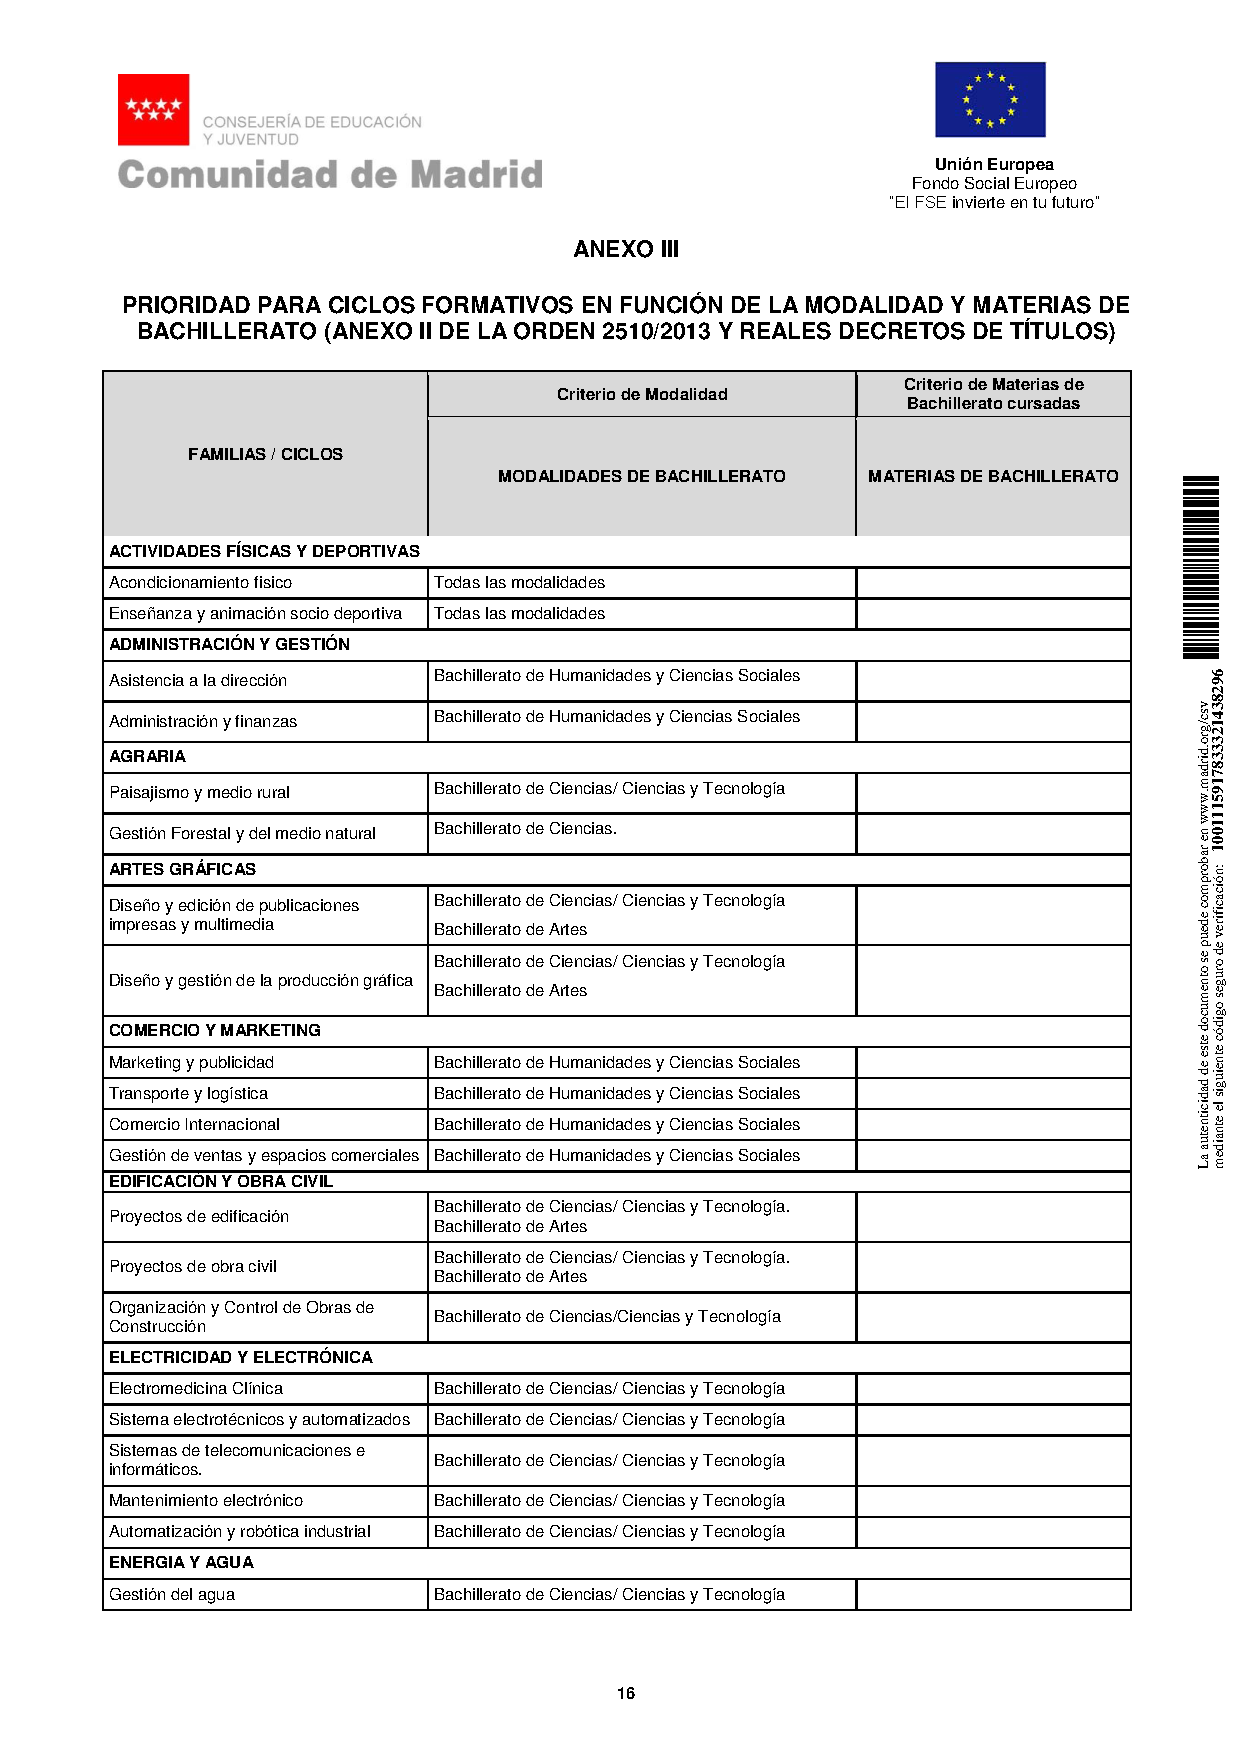
\includegraphics[width=.9\linewidth]{respuestas-posibles-preguntas/preferencias-anexo_iii_gs.pdf}
\end{center}
\end{NOTES}
\subsection*{Esto no es informática}
\label{sec:org0000027}
O al menos, es una parte muy pequeña


\subsection*{Cómo saber si me gusta}
\label{sec:org000002a}
>>>>>>> Stashed changes
\begin{itemize}
\item Programación: \href{https://scratch.mit.edu/}{Scratch} << \href{https://codecombat.com/}{Code Combat} << \href{https://www.aceptaelreto.com/}{Acepta el reto}
\item Bases de datos: \href{https://sqlpd.com/}{SQL Police Department} << \href{https://mystery.knightlab.com/}{SQL Murder Mystery}
\item Sistemas: \href{http://web.mit.edu/mprat/Public/web/Terminus/Web/main.html}{Terminus game} << \href{https://ubuntu.com/download}{Instalar linux}
\item Sistemas y redes: \href{https://overthewire.org/wargames/bandit/bandit0.html}{Bandit}
\end{itemize}
<<<<<<< Updated upstream
=======

\begin{NOTES}
\begin{itemize}
\item Inserción laboral
\item Porcentaje de aprobados
\end{itemize}
\end{NOTES}
\section*{Más información}
\label{sec:org0000030}
\begin{itemize}
\item Para volverlo a ver

\begin{center}

\includegraphics[width=.9\linewidth]{qr.png}
\end{center}

\item \href{respuestas-posibles-preguntas/madfpb-informatica-y-comunicaciones.pdf}{Básica}, \href{respuestas-posibles-preguntas/Ficha\_IFCM01-smr.pdf}{SMR}, \href{respuestas-posibles-preguntas/Ficha\_IFCS02-dam.pdf}{DAM}, \href{respuestas-posibles-preguntas/Ficha\_IFCS03-daw.pdf}{DAW}
\item \href{https://www.todofp.es/}{todofp.es}, \href{https://www.descubrelafp.org/}{descubrelafp.org}
\item \href{https://play.google.com/store/apps/details?id=org.madrid.fpmad\&hl=es\_ES}{Aplicación FPMad}
\end{itemize}
>>>>>>> Stashed changes
\end{document}
